\subsection{Классификационный подход к логотипу как способ его культурологического анализа}

В этом разделе мы сосредоточим свое внимание на четырех подходах к классификации логотипов:
\begin{enumerate*}[label=\arabic*)]
\item юридическом,
\item эмпирическом,
\item семиотическом.
\end{enumerate*}
Принципы отбора:
\begin{enumerate*}[label=\asbuk*)]
\item практическое назначение,
\item мотивы и темы,
\item степень суггестивного воздействия,
\item порождение значения.
\end{enumerate*}

В общем виде, классификация есть операция, заключающаяся в группировании определенного количества
фактов или явлений, обладающих общими характеристиками или признаками. В данном случае, предлагаемый
классификационный подход к систематизации практики лого дизайна преследует следующие цели:
\begin{enumerate}
\item Объединение логотипов в классы и группы согласно обозначенным принципам отбора.
\item Выявление сходств и различий в принципах, способах и приемах конструирования знака-образа коммерческого назначения.
\item Детализация композиции логотипа на примере его отдельных конкретных аспектов.
\item Определение роли исторических и социокультурных факторов в практической деятельности лого дизайнера.
\item Помощь в адекватном прочтении логотипа, анализе и интерпретации языка лого дизайна.
\end{enumerate}

В общем и целом смысл разработки такой классификации в создание материальной базы для последующей
разработки общей методологии анализа практики лого дизайна.

Ниже, как и прежде, мы будем двигаться от общего к частному и последовательно рассмотрим
официальные, эмпирические, семиотические, функциональные и авторские таксономии.

\subsubsection{Юридические, эмпирические, семиотические виды классификаций}

%% TODO: как всё-таки писать век?
Доподлинно неизвестно кто первым стал заниматься классификацией логотипов. Можно предположить, тем
не менее, что практическая потребность в классификации возникла, вероятно, с самого момента
зарождения торговых отношений, но стала по-настоящему актуальной только с развитием массового
производства. В конце XIX в., в 1883 г. Парижская конвенция об охране промышленной собственности
выделила товарные знаки из общего понятия клейм и признала их объектом исключительного права. В
Великобритании же <<Закон о регистрации торговых марок>> был принят ранее, в 1875 г., и вступил в силу
в 1876.

На сегодняшний день Всемирная организация интеллектуальной собственности (ВОИС) пользуется
специально разработанными классификационными системами, организующими информацию о изобретениях,
товарных знаках-логотипах и промышленных образцах, в индексированные, управляемые
таксономии. \autocite{vois} Самой распространенной системой является
Международная классификация товаров и услуг (Ниццкая классификация товаров и услуг для регистрации
знаков), которая состоит из 34 классов товаров и 11 классов услуг. Помимо Ниццкой
классификации, существуют также Локарнская, Венская и Страсбургская. Все логотипы (знаки) с
юридической точки зрения делятся на:
\begin{enumerate*}[label=\arabic*)]
\item товарные знаки,
\item знаки обслуживания,
\item коллективные знаки,
\item сертификационные знаки,
\item общеизвестные знаки.
\end{enumerate*}

Приоритетным для юридических схем классификации можно считать официальную регистрацию действующих и
планируемых знаков самоидентификации в целях обеспечения гарантий охраны права собственности. Таких
классификаций, по определению, может быть немного.

Напротив, неофициальных, стихийных классификаций логотипов существует довольно много. Они могут
носить неформальный характер, как, например, классификация Тибора Кальмана <<A New Identity>> для
журнала Print Magazine (2000) (см. Приложение~\ref{app:kalman}). Могут представлять собой
просто компилятивные подборки различных
видов графических символов, как в книге Elinor Selame из книги <<Developing a Corporate Identity>>
(1975). Наконец, могут использовать сложные комбинации структурирования материала, как в работе Пера
Моллерапа <<Marks of Excellence: The History and Taxonomy of Trademarks>> (1999). Так или иначе, все
исследователи, независимо от выделяемых категорий, склонны разделять логотипы по трём видам:
\begin{enumerate*}[label=\arabic*)]
\item Типографические или буквенные (logotype) (в основе слово)
\item Графические (картинные, иконические)
\item Смешанные или комбинированные (содержащие типографический и графический элемент).
\end{enumerate*}

Обратимся к примерам. Сначала компилятивные подборки.

В своей книге <<Торговые знаки и символы мира>> Ясабуро Кувайама разделяет их на четыре класса
(алфавит; конкретные фигуры; абстрактные фигуры; символы, числа и т. д.). Классификация Кувайамы
учитывает только материальные качества, а предложенные категории не являются ни взаимно
исключающими, ни исчерпывающими. Так, например, в книге <<Trademarks \& Symbols. Volume 1:
Alphabetical Designs>> (1973) Кувайама классифицирует логотипы в соответствии с буквами английского
алфавита A-Z. \autocite[][5]{kuwayama1973alphabetical}
Вторая книга <<Trademarks \& Symbols. Volume 2: Symbolical Designs>> (1973) включает
классификацию по мотивам и темам. \autocite[][5]{kuwayama1973trademarks}
В ней представлены логотипы основанные на: фигурах людей, лицах, глазах, руках, животных, птицах, рыбах, насекомых, цветах, деревьях, архитектуре, транспорте, стрелах, астрономических объектах и т.д.

В статье <<Типограф как аналитик>> Ганс Векерле\autocite{weckerle1968typographer} представил торговые марки в
симметричной матрице 9 x 9 (Вербальный символ: логотип; Вербальный символ: аббревиатура; Вербальный
символ: инициал; Графический символ: ориентированный на продукт; Графический символ: метафорический;
Знак: образный; Знак: цветной; Эмблема: персональная; Эмблема: общественная). Смысл использования
симметричной матрицы заключается в том, что многие торговые знаки попадают в более чем один
класс (см. рис.~\ref{fig:wekerle}).

\begin{figure}
  \centering
  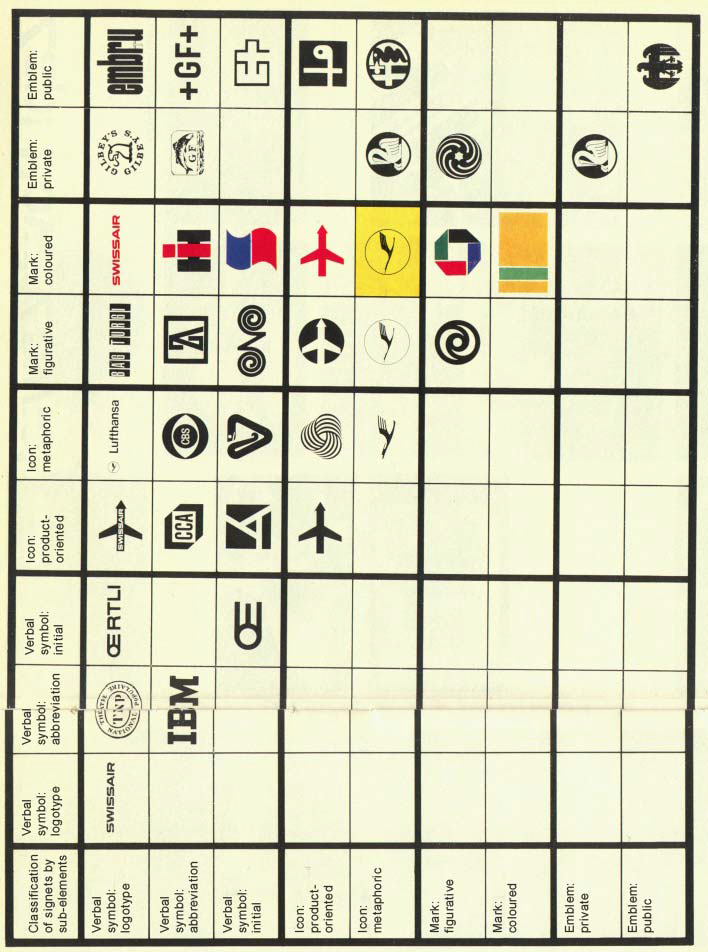
\includegraphics[width=.5\linewidth]{images/wekerle}
  \caption{Классификация Ганса Векерле: симметричная матрица 9 x 9}
  \label{fig:wekerle}
\end{figure}

В комментариях, редактор журнала Design Magazine писал: <<С середины 50-х годов начинается постепенный, хотя часто и совершенно произвольный переход к использованию абстрактных символов для идентификации компании. Они почти полностью вытеснили образные иллюстрации, которые, не смотря на малую информационную ценность, все-таки отличались гуманитарным реалистическим содержанием. Многие из новых символов уже утратили подлинный символический статус и лишены конкретного смысла.  Классификация Г. Векерле детализирует широкий спектр структурных элементов таких символов. Предельно точное описание природы индивидуальных знаков  позволяет создать более функциональный подход, как к  разработке, так и к практическому использованию символики компании, для разных типов предприятий и разных целевых установок.  На сегодняшний день – это первая точная классификация в данной области>>.

Как видим, авторы компилятивных сборников руководствуются главным образом интуицией и желанием найти
оптимальный функциональный принцип сведения всего многообразия логотипов к нескольким простым
доминантам, чтобы затем удобно расположить знаковые кластеры по правилу концентричности. Такие
классификации носят откровенно прикладной характер и ориентированы на то, чтобы быстро информировать
дизайнера, как любителя, так и профессионала, о положение дел в практике лого дизайна на данный
момент.

Более строгий, аналитический подход к классификации логотипов пока встречается крайне редко. По этой
причине любая попытка выйти за пределы наличной эмпирической данности и отрефлексировать накопленный
опыт всегда привлекает к себе особое внимание. Такой пионерской работой можно считать обстоятельное
исследование по истории торговых марок и графических символов П. Моллерапа, в которой он предлагает
семиотический взгляд на родовую классификацию знаков. Обобщив опыт предшественников и современников,
Моллерап подразделяет логотипы (торговые знаки), по признаку функциональности и суггестивной
действенности дизайна, определяя их материальные (то, что торговые знаки изображают) и референтные
(то, что торговые знаки означают) качества. Поговорим об этом чуть подробнее.

Любая классификация, согласно Моллерапу\autocite[][98]{mollerup1999marks}, чтобы соответствовать
своему целевому назначению, должна отвечать следующим критериям:
\begin{enumerate}
\item Идеальная классификация состоит из отдельных групп, между которыми есть чёткая
  граница. Классификация любого объекта должна быть понятна.
\item Критерии, согласно которым строится классификация, должны применяться одновременно. Каждый
  определяющий шаг классификации должен разделять объекты по какому-то одному единому принципу.
\item Выделенные группы одного уровня не должны пересекаться, то есть ни один объект не должен
  принадлежать более чем одной группе.
\item Все группы одного уровня должны охватывать всю совокупность объектов. Любой объект должен
  принадлежать какой-то группе.
\item Формирование групп должно быть обосновано с точки зрения цели построения классификации.
\end{enumerate}

Несмотря не очевидные достоинства такого продуманного подхода, на практике, таксономия, построенная
по этим критериям, как выясняется, объективно не может им следовать до конца. Трудности при
проведении процедур отбора и упорядочения возникают сразу по целому ряду направлений. Первое. Не
всегда возможно провести разделение между группами, т.е. первое и третье правила классификации
вынужденно нарушаются, чтобы выполнялось пятое. Второе. Невозможно установить однозначные границы
между всеми группами одного уровня. Соответственно, заявленные свойства логотипов далеко не всегда
ясны и эксплицитно выражены, а периодически, просто количественны. Третье. Буквы логотипа могут быть
настолько особенными по своей форме, что почти никто не узнаёт в них сами буквы. Объяснение, которое
придаёт смысл логотипу, может быть почти забыто, и для большинства пользователей логотип будет
неявным и даже нереалистичным. Однако свойство используются согласованно, и на каждом шаге
происходит деление только по одному признаку. Четвертое. Группы одного уровня могут
пересекаться. Логотип может содержать одну или несколько букв и картинку, поэтому может и
принадлежать сразу двум группам одного уровня одновременно. Наконец, возможны и другие комбинации
групп. Название может содержать и имя собственное, и обычное безличное имя существительное. Иными
словами, по каждому отдельно взятому свойству таксономия действительно позволяет чётко провести
разделение и упорядочение групп. В то время как на практике свойства, оправдывающие формирование
конкретной группы, зачастую не только не взаимоисключают друг друга, но и проявляются
одновременно. Один логотип может обладать свойствами, присущими двум или более группам.

Тем не менее, в совокупности группы одного уровня действительно покрывают все возможные логотипы
данной категории. Например, если логотип не является графическим, то он и не графический, и т
д. Другим достоинством классификации Моллерапа является тот факт, что она строится на логотипе как
таковом. На его материальных свойствах, на его связи с предметом обозначения, на его референтных
признаках, стилистической пластичности и способности превращения в аллюзию. На самом деле:
материальные свойства логотипа, скорее всего, примерно одинаково воспринимаются большинством
потребителей. При этом культура и культурный контекст, в котором потребитель встречает логотип,
могут значительно варьироваться, что влечет за собой вариативность интерпретаций и, тем самым,
вариативность приписываемых ему референтных качеств.

Из сказанного следует, что один и тот же логотип может быть классифицирован по-разному, и,
следовательно, все классификации логотипа в этой таксономии -- это лишь <<возможные>>
классификации. Номинально исходная классификация Моллерапа представлена двумя семиотическими
категориями (свойства), восемью критериями разделения, семью промежуточными и тридцатью конечными
группами таксономии (см. таблицу~\ref{tab:mollerup1}). Образно она показана в виде дерева
(см. таблицу~\ref{tab:mollerup2}) Корни: \emph{summum genus} -- группа, из которой вырастают надземная
часть дерева. Тринадцать ветвей вправо -- \emph{infima species} -- итоговые группы. В промежутке
находятся \emph{subaltern genera} -- промежуточные группы. Далее, акронимы, сокращения по начальным
и не начальным буквам могут быть дальше разделены как названия, на собственные имена, описательные
имена, метафоры, неочевидные имена и искусственные имена, но это, видимо, слишком. Большая часть
сокращений -- это нарицательные имена. (Подробнее см. \autocite[][98-123]{mollerup1999marks})
Остановимся здесь.

Итак:
\begin{enumerate}
\item Мы сделали краткий вводный обзор подходов к классификации логотипов по трем направлениям:
  официально-юридическому, неформально-эмпирическому и популярно-семиотическому.
\item Мы постарались показать сходство между этими подходами и проиллюстрировать различия.
\item Основная задача нашего изложения в этой части сводилась к тому, чтобы показать масштабность
  проблемы создания классификации логотипов вообще и создания единой объективной классификации в
  частности.
\item Важное здесь -- неизбежно эвристический характер создаваемых классификаций, их <<возможный>>
  статус. С одной стороны, это объясняется социокультурной обусловленностью чтения логотипов в
  практике жизни. С другой, спецификой деятельности лого дизайнеров, суть которой -- постоянный поиск
  новых идей.
\end{enumerate}

Одним источником вдохновения для лого дизайнеров являются сборники-классификации логотипов,
составленных самими дизайнерами. К разбору одного такого сборника мы и переходим.

\subsubsection{Авторские сборники-классификации}
\label{2.2}

%% TODO: и ещё одна путаница с веками.
На сегодняшний день одним из самых авторитетных сборников-классификаций логотипов в профессиональной
среде принято считать два тома визуальной хроники немецкой торговой марки <<A Treasury of German
Trademarks>> (1982, 1985), собранных американским шрифтологом и лого дизайнером Лесли
Кабаргой. Книги представляют собой себя собрание визуальных символов, логотипов, импринтов, обширную
картотеку торговых знаков, созданных в Германии во второй половине XIX в. -- первой половине XX
в. Первый сборник охватывает период с 1850-1925 гг., второй -- 1900-1950 гг.

Думается, выбор Германии в качестве объекта исследования в данном случае вполне закономерен,
учитывая то влияние, которое он оказал на мировую практику лого дизайна в ХХ веке. В совокупности в
сборниках представлены 600 знаков, созданных в Германии в указанный период. Многие логотипы показаны
в двух цветах, как они и были первоначально созданы. Ценность такой подборки, помимо сугубо
исторического значения, состоит и в том, что немецкие логотипы того времени по-прежнему продолжают
жить в современном лого дизайне в виде многочисленных заимствований, цитат, аллюзий, подражаний и
просто как пример красивых безупречно выполненных форм.

В содержательном плане классификация Кабарга включает в себя главным образом личные
идентификационные знаки известных дизайнеров или богатых влиятельных фирм, ценивших стильный дизайн
и имеющих достаточно средств на оплату услуг признанных немецких мастеров в этой области: Карл Шульпиг, Джозеф Биндер, Конрад Йоахим, Ф.Х. Эмке, Людвиг Хольвайн, Люциан Бернхард, Вильгельм Деффке и Карл Эрнст Хинкефус, Рудольф Кох, Вальтер Керстнг, О.Г.В. Хаданк, Филипп Зайц и др. Изобретательность, находчивость и остроумие именно этих дизайнеров Л. Кабарга кладет в
основу своей классификации. С другой стороны, именно эти качества побуждают современных лого
дизайнеров в обязательном порядке приобретать личную копию двухтомника, чтобы иметь ее всегда под
рукой.

Структурно материал сборника организован не по абстрактным категориям, как это обычно принято делать
в классификациях, а по персоналиям и тенденциям. Мы также последуем этому принципу ниже. Но для
начала выборочно представим наиболее ярких представителей немецкой школы лого дизайна.

\begin{enumerate}
\item \textbf{Фриц Хельмут Эмке} (1878--1965 гг.). Кроме создания логотипов, он, как и многие
  немецкие дизайнеры в те времена, занимался архитектурой, дизайном интерьера, плакатов, иллюстрации
  и разработкой шрифтов. Эмке даже придумал своё собственное слово для своих логотипов --
  <<kennbilder>>, которое приблизительно можно перевести, как мгновенно узнаваемая картинка; простой
  дизайн. Тот, который может рассказать историю при одном взгляде на него и при этом находить
  эмоциональный отклик у зрителя. Собственные дизайнерские находки Эмке, в свою очередь, были ни чем
  иным как откликом на орнаменталистику арт-нуво (рис.~\ref{fig:trademarks:german:emke}).
\item \textbf{Вильгельм Деффке} (1887--1950 гг.), \textbf{Карл Эрнст Хинкефус} (1881--1970 гг.). Оба
  дизайнера входили в ударную группу известной в Германии студии дизайна <<Вильгельмверк>> (1916--1920
  гг.), в начале столетия позиционировавших себя как наследников традиций старых немецких
  мастеров. Фирменный «черный» стиль немецкого лого дизайна сегодня -- наследие творческого успеха
  <<Вильгельмверк>> тех времен (см. рис.~\ref{fig:trademarks:german:dh}. В то же время, по
  исторической иронии, дизайнерская деятельность этой жеd студии косвенно ответственна за перерождение
  древнего символа жизненной энергии в нацистскую эмблему немецкого Рейха.
\item \textbf{Карл Шульпиг} (1884--1948 гг.) Один из наиболее часто копируемых немецких
  дизайнеров. Характерная черта его стиля -- органичное сочетание метафорического изображения товара
  с монограммной графикой в вербальной части знака. Возникающий эффект может носить легкий
  иронический характер, равно как и содержать ненавязчивый медитативный подтекст. Тем не менее,
  понять суть его подхода к дизайну непросто. Внешне неброский, стиль Шульпига требует даже от
  имитатора вдумчивого, вникающего отношения (рис.~\ref{fig:trademarks:german:shulpig}).
\end{enumerate}

%% TODO: и опять век!
Как мы уже отмечали, немецкие логотипы оказали большое влияние на визуальный язык XX века в целом. Германия начала XX века была экспериментальной площадкой для поиска новых нестандартных форм визуальной экспрессии,
принципов композиции и технологии производства. В этом смысле, можно было бы сказать, что самые
талантливые немецкие лого дизайнеры стали частью той широкой и неоднородной традиции, которая
позднее получила название модернизма, провозгласившего разрыв с предшествующим историческим опытом
художественного творчества. Стандартизация технологии производства, базовые принципы, такие как
<<принцип асимметрии, свободы от орнамента, ясности, соответствия духу времени, типографической
самодостаточности (``типографика – не живопись!'') остаются и сегодня в силе>>.\autocite[][8]{chihold2011}

Эстетический протест немецких графиков модернистов был направлен в первую очередь против засилья
тяжеловесных и вычурных форм уходящей эпохи, форм, трудных для быстрого прочтения и не
соответствовавших стремительному духу нового времени. Прежние приемы типографики ориентировались на
медленное, осмысленное прочтение сообщения. Соответственно, вопросы формы и эстетики при разработке
дизайна (выбор шрифта, орнаментов, сочетания шрифтов) имели приоритет перед утилитарной
функциональностью. Так, например, немецкие логотипы XIV-ХVII вв. типично включали в себя элементы
античной мифологии или геральдики -- королевские животные, щиты, мечи и различные комбинации простых
геометрических форм. Подразумевалось, что символическое наполнение логотипа по аналогии
воспроизводит символическое содержание ритуализованных знаков статуса и престижа. Как правило, они
были иллюстративны, сюжетны и описывали некое действо. Для примера: в ХVII в. Германии большой
популярностью пользовались массивные наружные вывески, содержащие реалистичное изображение. Так,
вывеска с именем купца -- Churchill дополнялась изображением церкви и поля, формируя расширенный
ассоциативный ряд для создания символического контекста восприятия знака. В тоже время, в городской
среде широкое распространение получили знаки-вывески прикладного, профессионально-ремесленного
назначения, представлявшие собой простые, стилизованные изображения какого-то ремесла или рода
занятий: очки -- врач-окулист, наковальня -- мастер-кузнец.

Напротив, главной стилеобразующей особенностью немецкого логотипа эпохи модернизма можно считать
выразительную лаконичность его формы и использование древних символов – молнии, креста, стрелы,
животного, птицы. Более того, в начале XX в. немецкая промышленость, ориентированная на массовое
производство товаров, придавала особое значение маркировке своей продукции посредством
логотипа. Часто такой знак был единственным визуальным элементом на упаковке и в рекламном
объявлении. Массовое производство, как отмечалось ранее, порождает массовый спрос, равно как и
создает условия для возникновения массового спроса на услуги лого дизайнера и способствует
формированию массовых профессиональных сообществ дизайнеров, как это и случилось в Германии --
<<Баухаус>>, <<Тотальный дизайн>>, <<Метадизайн>>. Для сравнения, американские логотипы того времени в
основном состояли из названий компаний написанных от руки или же стилизованных изображений
комических персонажей, таких как The Old Dutch Maid, Aunt Jemima, Rastus и
Mr. Peanut. \autocite{link:mpr} Лого дизайн как самостоятельный вид профессиональной деятельности
оформился в США гораздо позже, следуя заразительному примеру инновационного немецкого дизайна и
благодаря регулярным публикациям лучших работ немецких дизайнеров в авторских монографиях и
специализированных журналах, таких как <<Graphis>>, <<Gebrauchsgraphik>>, <<The Studio>>, <<Modern
Publicity>>. Возьмем для примера монографию типографа, дизайнера и педагога Яна Чихольда <<Новая
типографика>>\autocite{chihold2011}, в которой изложены базовые принципы модернистской типографики и
описан функциональный подход к оформлению печатных изданий.

Современный логотип, по Чихольду, должен быть простым и самобытным. Он должен легко запоминаться, то
есть быть узнаваемым и заметным. Как типограф, он убеждён, что хороший логотип совсем не обязательно
рисовать, поскольку эффективный товарный знак можно сделать и типографическим способом. Такой
логотип будет по определению функционален, и <<как и все вещи, выполненные при помощи техники, такой
знак несёт в себе заряд энергии>>\autocite[][118]{chihold2011}. И далее: <<Однако надо серьезно
предостеречь их от того, чтобы называть логотипом простую комбинацию литер из наборной кассы
(монограмму). Логотип -- это нечто совершенно иное, он вмещает в себя гораздо больше смысла, чем
простая монограмма, а плохой логотип гораздо хуже, чем его отсутствие. Сейчас типографы часто
соблазняются возможностью вместо прежних типографских виньеток печатать типомонограммы. Но в рекламе
нужны только логотипы; в наше время монограммы там бессмысленны. Монограмма в качестве фирменного
знака всегда хуже, чем логотип. А плохой логотип может испортить всю рекламную кампанию>>.
\autocite[][119]{chihold2011}

В виде программных требований -- своего рода манифест современного лого дизайна -- эта позиция
оформилась в 1929 году: <<1. Выразительность. Логотип должен выражать качество
продукта. 2. Простота. Логотип должен быть простой, потому что её необходимо будет воспроизводить в
любых размерах и в любой среде. 3. Оригинальность. Логотип не должен быть похожа на другие
трейдмарки. 4. Вневременность. Он не должна возникать из просто модных поветрий. 5. Правильный знак
– основа эффективной рекламы компани>>. \autocite{cabarga1982treasury}

Обращает на себя внимание тот факт, что процитированные слова, сказанные почти столетие тому назад,
по-прежнему звучат свежо и актуально. Представления немецких дизайнеров-модернистов тогда
практически не отличаются от ожиданий и требований к логотипу сегодня. В каком-то смысле, быть
современным всегда -- был, есть и будет главным принципом модернистского мировоззрения. И если
модернизм, в широком смысле, есть <<другое искусство>>, главной целью которого является создание
оригинальных произведений, то лого дизайн в своей модернистской версии -- это <<другой дизайн>>,
базирующийся на внутренней свободе, остраненном видении мира и новых выразительных средствах
изобразительного языка. Само слово \emph{дизайн} означает -- проект, план, замысел. В свою очередь
проект (projectum), следуя логике латинского языка, и вовсе означает -- брошенный вперед\autocite[][323]{serov2005}, что само
по себе роднит немецкий модернистский дизайн с современным ему футуризмом. Футуристы, как известно,
придумывали не только новые слова, профессиональный жаргон, но и язык афиш, и язык плакатов -- язык
рекламы. <<Реклама--– имя вещи\ldots Думайте о рекламе!>>, писал
В.В. Маяковский.\autocite{mayakovsky1959}

Функционализм лого дизайна, т.е. что утилитарно, удобно, то и красиво, естественным образом вытекает
из манифеста художественного объединения Баухаус (1919--1933 гг.), выпущенного в 1919 г. В манифесте, в
частности, провозглашалось равенство между прикладными и изящными искусствами, декларировалось
программное намерение повысить качество выпускаемой продукции в целях удовлетворения массовых
потребностей населения. Для этого промышленные товары нужно сделать красивыми, доступными по цене и
максимально удобными. Иными словами, функциональными.

Другой вопрос, конечно, что функциональная красивость предметов массового потребления, предлагаемых
дизайнерами-модернистами, все-таки не имманентна самому предмету. По сути дела, она свидетельствует
в первую очередь о вкусе и художественном чутье дизайнера.

%% TODO: и опять век!
Таким образом, европейский модернизм в первых двух десятилетиях ХХ века, с его энергичным
стремлением утвердить новые нетрадиционные начала в художественной практике, пропагандой
непрерывного обновления художественных форм и условности (схематизации) стиля, можно назвать первым
значимым источником вдохновения и ориентиром для практики авангардного лого дизайна сегодня. Вторым
важным источником следует назвать <<модерн>> (ар-нуво, югендстиль и т. д.), другое масштабное
направление в европейском искусстве на рубеже ХIХ-XX веков. Модерну свойственно стремление к
сочетанию художественных и утилитарных функций в создаваемых объектах, вовлечение в сферу
прекрасного всех областей деятельности человека, живой интерес к технологиям, отказ от прямых линий
и углов в пользу более естественных, <<природных линий>>. Расцвет прикладных искусств -- еще одна черта
модерна. В том числе и расцвет лого дизайна, как мы отметили ранее, разбирая примеры из сборника
Л. Кабарга.

Таким образом, в самом начале ХХ века логотип оформляется и закрепляется в культуре в виде
концептуального понятия. В современном лого дизайне можно найти достаточно примеров влияний, как
идеологии модернизма, так и философии модерна. В ХХI веке произошли существенные изменения в
техническом решении логотипов. Если раньше логотипы сначала чеканились и рисовались, затем
печаталась, то теперь их дизайн целиком и полностью зависит от того, какое программное обеспечение
для работы с графикой появляется на рынке компьютерных программ. Персональный компьютер как
технология самым решительным образом перестраивают практику графического дизайна и формируют новую
визуальную эстетику. Трудоёмкие зрительные эффекты, оптические иллюзии и сложные градиенты теперь
создаются щелчком мыши, быстро и точно.

Логотипы сегодня изготавливаются серийно и с учетом многочисленных перспективных
носителей. Соответственно повышаются требования к их полифункциональным возможностям. Так, они
должны хорошо читаться в любом диапазоне: в максимально крупных и минимально мелких размерах, любых
форматах и расширениях, включая иконки меню мобильного телефона, URL строки на веб-сайте. Это
касается в равной степени и логотипов в телевизионных программах и широкоформатных кинофильмах, а
также логотипов на любом печатном носителе. В отдельных случаях можно проследить, как
провозглашенная немецкими модернистами лаконичность визуального знака явно вытесняется стремлением к
интенсивной визуальной красивости модерна, наглядно иллюстрируя принцип единства и борьбы
противоположностей. Вместе с тем, как отмечает один из ведущих американских дизайнеров-модернистов
Р. Рэнд: <<You can’t criticize geometry. It’s never wrong.>> Действительно, канонические логотипы NBC,
CBS, PBS, Mobil и др., созданные дизайн студией <<Chermayeff \& Geismar>> еще в середине ХХ века не
подверглись существенным изменениям. Сегодня мы видим их точно такими же, какими они были 50 и более
лет назад.

Подведем черту.
\begin{enumerate}
\item В этом разделе мы вели речь о традиции классификационных сборников логотипов, составляемых
  практиками лого дизайна. Такие сборники, как правило, носят историографический характер и
  выполняют функции профессионального справочника, учебного пособия, документальной хроники
  становления традиции.
\item В качестве примера мы выбрали двухтомное издание американского дизайнера Л. Кабарга, в котором
  задокументирована почти столетняя история немецкой торговой марки (логотипа).
\item Помимо богатого иллюстративного материала, сборники Л. Кабарга содержат ценный
  культурно-исторический комментарий о деятельности немецких лого дизайнеров в контексте своего
  времени -- влияниях, заимствованиях, примерах сотрудничества и кооперации.
\item Мы говорили преимущественно о периоде на рубеже двух предыдущих веков, условно совпадающем с
  функционированием двух несовпадающих художественных направлений в искусстве -- модернизм и модерн.
\item Мы попытались показать, во-первых, как немецкие лого дизайнеры в начале ХХ века активно
  использовали визуальный язык, художественные принципы и приемы работы, характерные для того и
  другого направления. Во-вторых, мы предложили рассматривать современные логотипы, с одной стороны,
  как продолжение сформировавшейся традиции, и как ее преодоление, с другой.
\end{enumerate}

Теперь рассмотрим вопрос о классификации логотипов по темам и мотивам.

\subsubsection{Культурно-историческая классификация}
\label{2.3}

Одним из самых популярных способов классифицирования логотипов следует считать
организацию знаков по принципу ассоциативного ряда. Как правило, структурно
такая классификация представляет собой обширные тематические блоки,
внутри которых кластеры логотипов дифференцируются по тому или иному мотиву --
мифологическому, историческому, культурному, социальному и т.д. За неимением
специального термина мы называет такой подход классификации логотипов
культурно-историческим. Более того, составителями таких компендиумов визуальной
культуры обычно становятся историки и философы, как, например, в случае с
классификацией французских логотипов, разработанной историком Эдит Амиот и
философом Жан-Луи Азизола в 1990 г. и которую мы рассмотрим ниже. Также как
и в случае с авторскими сборниками логотипов, классификация Амиот и Азизола
не претендует на научную объективность. Границы между выделяемыми ими категориями
очень условны, и логотипа одного кластера можно с легкостью помещать в
другую рубрику по другому признаку отбора. Вместе с тем, их подход представляется
чрезвычайно плодотворным, во-первых, в своей познавательной части и, во-вторых,
в части обозначения топографического ареала символических потенций коммерческого
знака-образа. Итак, французский логотип в культурно-исторической перспективе.

С момента зарождения практики регистрации авторского права в 1857 году
Французским Национальным Патентным Бюро, их хранилища сегодня содержат
оригиналы всех зарегистрированных логотипов, счет которым уже давно перевалил
за миллион.

Для своей классификации Амиот и Азизола отобрали 2500
знаков. \autocite{edithjeanluois} Цель отбора --
показать эволюцию экономической деятельности французских корпораций за последние
150 лет в свете изменений социокультурного опыта повседневной жизни в обществе,
в той мере, в какой они отражены в практике графического дизайна в конкретный
исторический период. Материал организован по тематическому принципу. Всего таких
тем -- 27. Внутри каждой темы авторы, помимо представления иллюстративного
материала, предлагают свой комментарий о том, как, по их представлению,
знак-образ суггестивно воздействуют на потребителя. Перечень тем выглядит так:
античность; мифология; аллегории; нечисть; фольклорные персонажи; исторические
личности; Книга Бытия и святые; звезды; растительность; домашние животные;
лесные обитатели; дикие животные; птицы; рыбы; страны; регионы; архитектура;
изображение человека; дети, мужчины, семейные пары; женщины; юмор; предметы и
материалы; антропоморфизмы; труд; транспорт; графичность.

Примечательно, что в классификацию не вошли логотипы-названия фирм, за исключением
тех, которые используют уникальную каллиграфию. Авторы объясняют это тем,
что именно визуальный язык является тем доминирующим фактором, который определяет
качество и надежность <<отпечатка>> в памяти потребителя. В концентрированном виде
логотипы выражают эмоционально окрашенное культурное содержание --
национально-специфичные архетипы коллективной памяти, универсальные символы и
представления о мироздании, понятные всем. По этой причине в лого дизайне
утвердились традиционные темы и мотивы композиции -- сказочные герои, животный
и растительный мир, патриотические сюжеты, призванные помочь установить мгновенную
ассоциативную связь между изображением и припоминаемым (узнаваемым) ассоциативным
комплексом приятных ощущений в лимбической системе головного мозга потребителя.

Связь эта непрямая и в разных случаях призвана решать разные задачи идентификации.
Иногда она может строиться на метафорической связи изображаемого со специфической
деятельностью компании или ее продукцией. Например, логотип компании <<Lacoste>>,
производящей одежду, обувь, парфюмерию и т.д., содержит изображение аллигатора.
Метафора, напомним, это скрытое сравнение, имеющее трехчленную структуру:
\begin{enumerate*}[label=\asbuk*)]
    \item что сравнивается,
    \item с чем сравнивается,
    \item на каком основании сравнивается.
\end{enumerate*}
В нашем случае, предлагается сравнить и обнаружить сходство между водным
позвоночным и деятельностью (продукцией) компании. Основание для сравнения
предлагается сделать самому потребителю. Желаемый ассоциативный ряд, по-видимому,
будет включать абстрактные качества по схеме <<компания такая же\ldots как аллигатор>>.
Например, энергичная, мощная, цепкая, надежная и т.д. Или: наши изделия из
кожи такие же прочные (экзотичные, престижные и т.д.) как кожа аллигатора. Далее,
компания Lacoste не только идентифицирует себя через данную визуальную метафору.
На следующем этапе она предлагает сознанию массового потребителя принять ее
как данность, т.е. перейти от операции сравнения к операции отождествления
желаемого основания для сравнения с именем (имиджем) самой компанией. Метафорические
связи уступают место символическим, метафора трансформируется в символ и миф в
массовом сознании.

Следует заметить, однако, что для знатоков и поклонников тенниса, а именно -- тех,
кто доподлинно знает историю возникновения логотипа Lacoste, знак-образ, с одной
стороны, лишен какой бы то ни было отвлеченной метафоричности. Изображение
аллигатора есть всего-навсего визуальная шутка. Lacoste -- это имя основателя
компании Жана Рене Лакоста, знаменитого французского теннисиста в перво
й половине ХХ века. Во время кубка Дэвиса в 1927~г. капитан французской
сборной по теннису пообещал Рене Лакосту крокодиловый чемодан за победу на турнире.
Турнир он проиграл, но американская пресса мгновенно окрестила Лакоста <<аллигатором>>.
Прозвище закрепилось и даже получило одобрительную символическую интерпретацию,
описывающую его упорное и цепкое поведение на корте. Аллигатор позднее в качестве
личной эмблемы был вышит на блейзере, в котором выступал Лакост. Следовательно,
в сознании потребителя товаров компании Lacoste изображение аллигатора
отождествляется с легендарным теннисистом, становится символом успеха, славы и
престижа. На языке маркетинга -- обещание ценного приобретения, ценности как
таковой, т.е. бренд. Бренд -- это обещание потребного будущего по архаической
суггестивной формуле: <<если\ldots то>>. Если вы будете приобретать наши товары,
то ценные качества, успех и слава героя спорта перейдут к вам.

Соответственно, в классификации Амиот и Азизола обычные знаки-образы прагматичной
самоидентификации объединяются со знаками-образами символического
самоотождествления. К последним следует отнести логотипы, ассоциативно усиливающие
ностальгическое переживание культурно-исторического прошлого как более
простого времени, времени более интересного, более нравственного, более
героического и т.д. Ведь логотипу, как и рекламе вообще, совершенно необязательно
показывать сам товар или его производителя. Достаточно создавать настроение,
которое оттеняло бы их привлекательность и вызывало положительные эмоции.
В этом смысле, логотипы создают мемы-ассоциации, формирующие положительное
отношение к деятельности компании и ее продукции. Они продают чувства,
с одной стороны, и обещания привлекательного статуса, с другой. Выборочно
рассмотрим культурную составляющую классификации Амиот и Азиола и снабдим кратким
комментарием. Выделяемые блоки: Античность, Животный и растительный мир, Части света, Изображение человека.

\paragraph{Античность}
Античный стиль очень гармоничный и всегда являлся эталоном для подражания.

Ассоциативная привлекательность образов в их престижности, величественности,
авторитетности, долговечности, историчности и т.д.

\emph{Вавилон}. В 1925 году магазин одежды <<A la ville de Babylone>> выбрал в качестве своего логотипа крылатого быка с человеческой головой, статуи которого когда-то охраняли вход в город в
  Месопотамии (рис.~\ref{fig:trademarks:french:1.1}).  Знак -- точная копия скульптуры быка, хранящейся в
  Лувре. Аналогично, в 1969 году Дом Ирана в Париже взял в качестве своей эмблемы образ двукрылого
  сфинкса, точную реплику барельефа на покрытом эмалью кирпиче архимедианской эпохи, также хранящемся
  в Париже (рис.~\ref{fig:trademarks:french:1.2}).
  
\emph{Греция и Рим}. Культ олимпизма и античных пластических форм как тема лого дизайна вошли в моду
  благодаря Олимпийским играм, проводившихся в Париже в 1924 году. Прославленная красота богинь,
  аскетизм и суровость древних греков и римлян, их несгибаемый дух боевого соперничества породили
  целый вихрь образов, чья красота выражала идею совершенства, мужества, благородства и
  сдержанности. Или более приземленно: Афина Паллада продает пиво (рис.~\ref{fig:trademarks:french:2.3}),
  Пан, бог пастушества и скотоводства используется в качестве торгового знака для продажи сыра
  (рис.~\ref{fig:trademarks:french:2.11}), Аполлон убивающий стрелой
  змею на логотипе фармацевтической лаборатории утверждает их намерение покончить со злом в виде
  болезней (рис.~\ref{fig:trademarks:french:2.10}).

\paragraph{Животный и растительный мир}

В дизайне логотипов зачастую используются изображения растений, животных и птиц,
как цельные формы, так и их метонимические атрибуты. Например, крыло, рога,
силуэты или тени, оттенки шкур. Наиболее распространены символические изображения
животных и птиц, так как у человека в ходе истории сформировались определенные
ассоциации с тем или иным животным, птицей или растением.

\emph{Растения}. Ассоциативная привлекательность образов в их совершенной
  красоте, символическому отождествлению с христианскими добродетелями,
  гармоничностью, выразительностью, стремлением к совершенству, плодородием,
  ростом и т.д.

  Так, в лого дизайне образ трехлистного клевера, символа Троицы, становится
  символом денег, а четырехлистный клевер символом удачи
  (рис.~\ref{fig:trademarks:french:9.14}). Мотив листа с прожилками часто
  представляет дистрибуционную сеть для сельскохозяйственных продуктов. Цветы
  также способны образовывать прочные связи между товарами, которые они
  представляют, и потребителями. Например, цветочные орнаменты эпохи Арт Деко
  (рис.~\ref{fig:trademarks:french:9.21}) использовали на мотиве розы.  В
  гирляндах или в качестве бутоньерок розы символизирует природную женскую
  элегантность. Образ дерева, с другой стороны, это прочная опора, в которой
  циркулирует жизненная энергия. Эмблемы, основанные на символе дерева,
  подчеркивают его силу и символическую идею подлинности и уверенности.

\emph{Животные}. Ассоциативная привлекательность образов в безграничных
  возможностях символизации, таких как ощущение тепла и нежности, идеи изобилия и
  плодовитости, качества сообразительности, силы и быстроты, чувства радости,
  веселья, страха и т.д.

  Мотивы животных выделяются едва ли не в каждой книге, посвящённой дизайну
  логотипов. Они легко запоминаются и по этой причине помогают продавать все что
  угодно, как, например, логотип с <<курящим кроликом>>, продающим сигаретную бумагу
  (рис.~\ref{fig:trademarks:french:10.5}). Известные своей плодовитостью, зайцы и
  кролики обещают изобилие компаниям, выбравшим их для своих логотипов.  Из
  домашней птицы: цыплята символизируют детство, а куры -- материнскую опеку.
  Образ петуха -- самый частотный во французском лого дизайне. Петух также
  является национальной эмблемой Франции, а в функции флюгера на вершине
  церковного шпиля становится величественным выражением патриотического
  единства. Графика изображения французского петуха менялась с течением времени,
  но его можно было всегда опознать по гребню и характерным серповидным перьям в
  хвосте (рис.~\ref{fig:trademarks:french:10.51}).

  Из других предпочтений: За коровами прочно закрепилась ассоциация с молочными
  продуктами. Исключение составляет успешная марка плавленого сыра <<Vache qui
  rit>> (Смеющаяся корова). (рис.~\ref{fig:trademarks:french:10.90}). Логотипы с
  изображением овец обычно использовались для продажи текстильных изделий. Собака
  может олицетворять преданность, соперничество и элегантность
  (рис.~\ref{fig:trademarks:french:10.131},
  рис.~\ref{fig:trademarks:french:10.138}).  Образ запасливой белки часто
  используется для продажи консервированных продуктов, в то время как еж помогает
  продавать товары для садоводства (рис.~\ref{fig:trademarks:french:11.6}).
  
\emph{Птицы}. Ассоциативная привлекательность образов в эстетичности,
  экзотичности, идее полета, свободы, изменения, возрождения и т.д.

  По статистике из всего животного мира именно птиц выбирают чаще всего для
  того, чтобы представить продукт или брэнд. Знакомые виды и экзотические,
  неуловимые и хрупкие, они могут иллюстрировать качества столь противоположные,
  как деликатность и власть. Птичий полет легко представить символом отношений
  между небом и землей. Они олицетворяют собой мечту и освобождение от земных бед
  и неурядиц. У каждого вида свое символическое назначение.  Трясогузка
  (рис.~\ref{fig:trademarks:french:12.1}) ассоциируется с любовным томлением и
  древнегреческими любовными зельями. Ласточка символизирует изменение,
  возрождение и плодовитость (рис.~\ref{fig:trademarks:french:12.2}). Морская
  чайка напоминает нам об океане. Плутоватая и болтливая сорока иллюстрирует идею
  баловства (рис.~\ref{fig:trademarks:french:12.12}) , а голубь символизирует идею
  чистоты души.
  
\paragraph{Части света}

 Части света -- регионы суши, включающие материки или их
  крупные части вместе с близлежащими островами. Принято выделять шесть частей
  света. Ниже мы говорим только о двух.
  
\emph{Азия}. Ассоциативная привлекательность образов в экзотичности цветовых
    гамм и восточных мотивов.

    Появление восточных мотивов во французском лого дизайне совпадает с началом
    проведения Всемирных Ярмарок в Париже (1855), на которых экспонировались
    экзотические товары и экспонаты из Азии, достижения колониальной экспансии
    Франции. Только в ХIХ веке в Париже прошло шесть таких ярмарок. Среди логотипов,
    вдохновленных Азией, в основном преобладали японские цветочные мотивы
    (рис.~\ref{fig:trademarks:french:15.9}), женщины в кимоно, китайцы в
    конусообразных шляпах.  Использовались такие мотивы в рекламе парфюмерных
    товаров, кулинарных специй и пряностей. %(Пример!)

\emph{Африка}. Ассоциативная привлекательность образов в экзотичности далеких
    стран и цивилизаций.

    Если идеализированные образы символизирующие Восток традиционно поэтичны, то
    первые логотипы, изображающие африканцев, носят подчеркнуто расистский
    характер. Широкое распространение получили обезьяноподобные образы чернокожих
    рабов (рис.~\ref{fig:trademarks:french:15.29}), обряженных в полосатую одежду
    или униформу.  Отношение начинает меняться в 30-е годы ХХ века, в связи с
    нарастающей популярностью американского джаза во Франции. Способствуют этому
    также и научные экспедиции в Африку, открывшие широкой публике глаза на
    самобытность и оригинальность африканского искусства и культуры.  Наконец, успех
    движения за права чернокожих в США (1950-е~--~1960-е) приводит к решительной
    смене настроений в обществе. В лого дизайне на смену образам большегубых
    негритянок приходят атлетически сложенные чернокожие красавицы
    (рис.~\ref{fig:trademarks:french:15.47}) . Колониальные мотивы в дизайне
    окончательно вытесняются экзотикой другого толка: очарованием далеких незнакомых
    цивилизаций. Зачастую эти мотивы использовалась для продажи ширпотреба: одежды,
    шоколада, мороженого и т.д., постепенно превращаясь в обычные китч-образы,
    свойственные массовой культуре как таковой %(Пример!).

  \paragraph{Изображение человека} 
  
  Изображение человека в логотипе делает его более приветливым, доброжелательным, дружелюбным и таким образом говорит об ориентации в своей работе на человеческий фактор. Такие изображения могут использовать на
    логотипах социальных учреждений, кафе и т.д.
 
     \emph{Дети}. Ассоциативная привлекательность образов в удовлетворении
      ностальгической потребности взрослых в воспоминаниях детства и потребности детей
      в образцах для подражания.

      Детство -- беспечная пора в жизни человека, ассоциируемая с безусловной
      материнской любовью (рис.~\ref{fig:trademarks:french:20.22}) и беззаботными
      играми (рис.~\ref{fig:trademarks:french:20.23}). На детей младшего возраста
      воздействуют образы старших подростков. Они стремятся скорее стать взрослыми,
      добиться признания и уважения у друзей и родителей. Положительную реакцию у
      детей постарше и у подростков вызывают образы кумиров -- известных футболистов,
      музыкантов, или актеров, которым они стремятся подражать.

   \emph{Мужчины}. Ассоциативная привлекательность образов в удовлетворении
      идеальных представлениях о мужественности и семейных отношениях.

      Логотипы с изображениями мужчин в прошлом ориентировались на стереотипные
      представления о мужественности. Мужчины здесь мускулинизированы, полны
      внутренней энергии и решимости. (рис.~\ref{fig:trademarks:french:20.4})
      Мода ХIХ века диктовала мужчинам необходимость выглядеть солидно и
      импозантно. Напротив, современные логотипы часто ассоциируют мужчин с
      предметами роскоши или исключительными предметами, такими как складной
      цилиндр (рис.~\ref{fig:trademarks:french:20.7}). Считается, что новый тип
      мужчины полагает, что, потеряв внешний лоск, он компенсирует это ощущением
      истинной силы. Его жена или подруга становятся показателем его достатка и
      вкуса, в той мере, в какой он проявляется в ее красоте и нарядах. По это
      причине современные мужчины на логотипах нередко изображаются в компании
      привлекательных женщин (рис.~\ref{fig:trademarks:french:20.21}).

  \emph{Женщины}. Ассоциативная привлекательность образов в демонстрации
      идеальных образцов женской красоты и совершенства, грации и пластики,
      элегантности и роскоши, и т.д.

      Образы женщин традиционно представляют бренды, ориентированные
      на предложение товаров для женщин -- гигиенических средств, косметики, средств
      ухода за волосами, женского белья и проч. В исторической перспективе изменения в
      предложении позволяют проследить этапы развития женской моды, равно как и этапы
      женской эмансипации. Скажем, если женское белье относится к области потребления
      товаров личного или интимного назначения, то такие аксессуары, как макияж и
      духи, участвуют в формировании имиджа женщины на публике. В качестве примера:
      кокетки ХVIII века придумали особый язык мушек, которым активно пользовались как
      орудием флирта. Аналогичную функцию выполняли макияж и духи. В двадцатые годы
      прошлого века женщины начали публично красить губы. Алые губы мгновенно
      появились на логотипах. Самый знаменитый пример -- <<Красный поцелуй>> (риc.~\ref{fig:trademarks:french:21.32}),
      логотип фирмы по производству губной помады. Наконец, образ женщины на отдыхе
      или на работе также повсеместно использовался в лого дизайне. Для продвижения
      бытовых товаров изображались женщины в простых, будничных ситуациях (риc.~\ref{fig:trademarks:french:21.34},
      риc.~\ref{fig:trademarks:french:21.53}). Часто такие логотипы имеют эффект снимка, фотографии. В логотипах одежды
      от кутюр и напитков, наоборот, используются силуэты прекрасных дам. Застывшие
      жесты и торжественные позы символизируют моду и роскошь
      (риc.~\ref{fig:trademarks:french:21.45}, риc.~\ref{fig:trademarks:french:21.52}). Среди
      логотипов этого направления много реалистичных изображений женщин, выполненных в
      стиле эпохи их создания.

Таким образом, мы произвели выборочный разбор классификации логотипов по
культурно-историческому принципу на примере классификации французских
логотипов историком Эдит Амиот и философом Жан-Луи Азизола. Смысл такой
классификации не ограничивается ее культурно-исторической направленностью.
Она также имеет важное практическое значение, поскольку непосредственно
влияет на качество образования и формирования индивидуального графического
стиля современного лого дизайнера. Понятно, что какие-то мотивы, отраженные
в классификации, вышли из употребления вместе с уходом своего времени.
Например, изображение автомобиля вряд ли сегодня может представить в качестве
символа передовой технической мысли. Другие продолжают функционировать,
такие как, например, изображения мифологических существ, животных, растений,
рыб, человека и т.д. Важно то, что логотип здесь представлен полноценным
знаком культуры, документирующим историю не только отдельно взятых компаний,
но и историю определённого исторического периода истории страны. Как и
современный логотип, он отображает ментальность людей, их потребности,
желания и нравы.

Разумеется, в лого дизайне есть примеры и других классификаций,
организующие знаки по их исторической социокультурной наполняемости, как,
например, недавно переизданная коллекция логотипов Эрика Бейкера и Тайлера
Блика <<American Trademarks: From the Roaring '20s to the Swinging '60s>>. \autocite{bakerblik2010}
Это основательная подборка знаков организована тематически по категориям:
дамы и господа, животные, транспорт, круги и формы, ковбои и индейцы,
типографика и, наконец, лица и фигуры. Логотипы учитывают предмет, тему и
форму знака, и предлагают дизайнерам и поклонникам <<американского стиля>>
возможность окунуться в прошлое графического дизайна. Новое издание книги
включает более 1500 известных и менее известных логотипов с 20-х годов
прошлого века и далее, включая современные марки и комментарии известных
дизайнеров. Далее, большой популярностью в профессиональной среде пользуется
двухтомное издание <<Famous Animal Symbols>> (1991) бельгийского дизайнера Пола
Ибоу.\autocite{ibou1991}
Том 1 содержит 266 логотипов животных, получивших мировое признание, и
созданных, по большей мере, профессиональными и хорошо известными художниками,
графическими дизайнерами и рекламными агентствами. Том 2 -- более 250. Тем не
менее, мы остановили свой выбор на историко-культурологической классификации французских логотипов как наиболее полной, детальной и ориентированной на широкий круг
заинтересованных читателей.

Подведем общий итог.
\begin{enumerate}
\item При рассмотрении вопроса о классификации логотипов мы исходили из той
  эмпирической данности, что единой общепринятой классификации коммерческих
  знаков идентификации на данный момент не существует.
\item Трудности создания такой классификации закономерны. Во-первых, сфера
  деятельности лого дизайнера находится в состоянии постоянного обновления и
  изменения. Во-вторых, эклектичный характер технологии создания логотипов
  существенно осложняет процесс отбора общих единых признаков, необходимых для
  формулирования принципов систематизации.
\item Существующие классификации логотипов различаются по функциональному
  назначению, полноте, авторству и принципам систематизации. Большинство
  наличных классификаций созданы для решения практических задач -- закрепление авторского права, обобщение опыта, установление исторической
  преемственности, описание достижений лого дизайна, определение корреляции
  производства логотипов с изменениями в социальной структуре массового
  общества.
\item Разделы \ref{2.2} и \ref{2.3} содержат разборы двух подходов к
  классификации логотипов, обобщающих опыт дизайнерской деятельности в
  Германии и Франции соответственно. В разборе немецкого опыта мы обратили
  внимание на попытку автора поместить деятельность лого дизайнеров начала
  ХХ века в контекст двух широких влияний -- модернизм и модерн. Обе тенденции
  отчетливо прослеживаются в практике лого дизайна сегодня. В разборе
  французского опыта акцент был сделан на культурно-исторический аспект
  изображений на логотипах, популяризирующих те или иные символически насыщенные
  знаки по принципу создания ассоциативных рядов.
\item Мы также предложили различать разные уровни прочтения
  логотипа. К таковым мы отнесли
  \begin{enumerate*}[label=\asbuk*)]
  \item метафорическое прочтение, в основе которого лежит операция
    установления внутреннего сходства по какому-то одному признаку и
  \item символическое прочтение, в основе которого лежит операция
    отождествления знака с тем или иным ассоциативным комплексом.
  \end{enumerate*}
  В первом случае речь идет об игровом отношении к знаку, во втором -- о
  мифотворческом. Обе операции могут находиться в отношениях дополнительности.
\item Наконец, мы уточнили и расширили свое прежнее определение бренда,
  понимаемого как возможное символическое содержание логотипа. Теперь мы
  предлагаем считать бренд суггестивным символом, ориентированным на потребное
  будущее, обещающим значащее повышение качества жизни и самооценки потребителя
  через приобретение рекламируемого товара.
\end{enumerate}
